\section{Introduction}
\label{sec:intro}

Tokenization is often treated as a benign preprocessing step.
In professional structured and semi-structured classification pipelines, performance matters, but it must be delivered under hard throughput, latency, and context-length constraints.
Under these deployment constraints, tokenization is not merely formatting: it is a fixed \emph{representation interface}.
Inputs are deterministically serialized into strings and segmented into tokens, after which all downstream computation is conditioned on the token sequence.
Many such systems use encoder-style discriminative models for efficiency, but the central object here is the interface itself: changing the tokenizer changes the contract between raw symbolic inputs and the model, and therefore changes which distinctions can \emph{ever} be represented, learned, and recovered under binding token budgets.

Structured and semi-structured streams make this interface problem acute.
Their semantics is role- and boundary-dependent: the same character substring may be a key, a delimiter, or a value depending on its position and surrounding syntax.
They also contain high-cardinality fields (identifiers, timestamps, hashes, URLs) whose internal character patterns are unstable but whose span integrity is task-critical.
Under deterministic left-to-right, prefix-emitting execution, tokenization induces a causal mapping from raw prefixes to tokenized prefixes.
We call the resulting failure mode \emph{prefix semantic collapse}: two raw prefixes that correspond to different task-relevant semantic states become indistinguishable because they map to the same observable token prefix.
Collapse is an interface property: once it happens, no downstream encoder operating under the same tokenizer can reconstruct a distinction that never reaches the model, regardless of model size or training recipe.
This is especially damaging for streaming or early-decision settings and for any deployment with hard maximum sequence lengths.

Canonical tokenizers fail on structured inputs in a structural way.
WordPiece~\cite{schuster2012japanese,wu2016gnmt} and BPE~\cite{gage1994new,sennrich2016neural} optimize subword statistics largely driven by natural language, without constraints that respect role boundaries or typed value spans.
As a result, they may segment across boundary-bearing symbols, entangle role cues with incidental value fragments, and become brittle to semantics-preserving re-serialization (e.g., benign field reordering, whitespace/escaping normalization).
Conversely, using finer-grained pieces to avoid brittleness often leads to heavy-tailed token lengths on high-cardinality fields, inflating attention cost and truncation risk.
These effects are consistent with broader evidence that tokenizer choice and granularity can materially affect downstream behavior and robustness~\cite{rust2021good,bostrom2020byte,mielke2021between}.

These interface effects appear immediately under standard encoder limits.
In a scan of six widely used pretrained tokenizers on 5{,}000 CSIC 2010 HTTP requests~\cite{torrano2010csic} with $L_{\max}{=}512$, average sequence lengths range from 359--468 tokens and 7--29\% of examples exceed the limit (29.4\% for BERT WordPiece; 7.3\% for a GPT-3.5/GPT-4-family tokenizer; Table~\ref{tab:e0_tokenizer_playground}).
The tail is heavy: the longest request reaches 1{,}034 tokens, illustrating that truncation risk is an interface property of segmentation rather than a modeling detail.
Many widely deployed GPT-family tokenizers are also BPE-derived and inherit similar interface trade-offs~\cite{radford2019language,brown2020language}.

% \begin{figure}[t]
% \centering
% \begin{tokviz}
% \tok{GET}\tok{\detokenize{ }}\tok{/}\tok{search}\tok{?}\tok{q}\tok{=}\tok{\detokenize{%}}\tok{E7}\tok{\detokenize{%}}\tok{82}\tok{\detokenize{%}}\tok{B8}\tok{\detokenize{%}}\tok{E9}\tok{\detokenize{%}}\tok{B8}\tok{\detokenize{%}}\tok{A1}%
% \tok{\&}\tok{token}\tok{=}\tok{a}\tok{B}\tok{1}\tok{!}\tok{x}\tok{Y}\tok{9}\tok{@}\tok{z}\tok{Z}\tok{2}\tok{\#}%
% \tok{\&}\tok{id}\tok{=}\tok{0}\tok{x}\tok{7}\tok{f}\tok{8}\tok{e}\tok{9}\tok{a}\tok{0}\tok{b}\tok{2}\tok{c}\tok{4}\tok{d}\tok{\detokenize{ }}\tok{HTTP}\tok{/}\tok{1.1}\\
% \tok{Host}\tok{:}\tok{\detokenize{ }}\tok{127.0.0.1}\tok{:}\tok{8080}\\
% \tok{X-Trace-ID}\tok{:}\tok{\detokenize{ }}\tok{550e8400}\tok{-}\tok{e29b}\tok{-}\tok{41d4}\tok{-}\tok{a716}\tok{-}\tok{446655440000}\\
% \tok{Cookie}\tok{:}\tok{\detokenize{ }}\tok{sess}\tok{=}\tok{q}\tok{Wer}\tok{Ty}\tok{Ui}\tok{Op}\tok{12345}
% \end{tokviz}
% \vspace{-0.3em}
% \caption{Token-boundary visualization for a representative semi-structured request under a canonical WordPiece tokenizer (BERT family). Colors indicate token boundaries. The segmentation fragments boundary-bearing symbols and high-cardinality fields into many short pieces, obscuring role/value structure and inflating effective token budget.}
% \label{fig:intro_token_example}
% \vspace{-0.8em}
% \end{figure}

We therefore treat tokenization for structured prediction as a constrained interface design problem.
We introduce \emph{directed semantic distortion}, a prefix-aligned measure of irrecoverable task-relevant information loss incurred when prediction must be made from tokenized prefixes rather than raw prefixes.
This yields a deployment-aligned rate--distortion view of tokenizers under vocabulary and sequence constraints.
Building on this formulation, we propose \textbf{Controlled Interface Tokenization (CIT)}: a deterministic tokenizer that (i) enforces an explicit, versioned interface contract with role-preserving boundaries and typed-value integrity, and (ii) constructs task-specialized vocabularies by maximizing compression gain within the contract-feasible space under deployed prefix-emitting execution.

\paragraph{Contributions.}
Our contributions are:

\begin{itemize}
  \item We identify \emph{prefix semantic collapse} as an interface failure mode for structured streams: distinct task-relevant prefix states become indistinguishable after prefix-emitting tokenization, creating irrecoverable information loss under any downstream encoder.
  \item We propose \emph{directed semantic distortion}, a prefix-aligned, task-relevant measure of interface-induced information loss, enabling empirical rate--distortion analysis for tokenization interfaces.
  \item We introduce \textbf{CIT}, a contract-constrained, deterministic tokenization system that preserves role boundaries and typed-value integrity while inducing deployment-aligned vocabularies under prefix-emitting execution.
  \item We empirically validate a causal chain from interface to learning to system behavior: CIT avoids collapse on a synthetic prefix stress test, improves end-to-end learning and drift robustness under token-fair training on a public HTTP benchmark, and shifts the accuracy--latency Pareto frontier under fully trained encoder models.
\end{itemize}


The remainder of the paper develops the interface formulation, presents CIT, and evaluates its efficiency, robustness, and end-to-end impact under strict drop-in constraints.
Additional proofs and extended context are provided in the supplementary appendix.

\section{Related Work}
\label{sec:related}

\paragraph{Subword tokenization and robustness.}
Modern tokenizers for neural text models are typically learned subword segmenters, including WordPiece~\cite{schuster2012japanese,wu2016gnmt}, BPE~\cite{gage1994new,sennrich2016neural}, and Unigram/SentencePiece~\cite{kudo2018subword,kudo2018sentencepiece}.
While effective on natural language, their merges are largely frequency-driven and can be brittle under distribution shift or when task semantics depend on non-linguistic boundaries.
Prior work has documented that tokenizer choice and granularity can materially affect downstream accuracy and robustness, even with the same model family and training recipe~\cite{rust2021good,mielke2021between,bostrom2020byte}.
Our work complements these studies by focusing on structured streams and by making the \emph{prefix} irreversibility of interface failures explicit.

\paragraph{Byte-level and token-free interfaces.}
Token-free modeling at the byte or character level avoids segmentation errors and preserves all raw information, but typically increases sequence length and compute~\cite{xue2022byt5,clark2022canine,yu2023megabyte}.
These approaches trade semantic fidelity for rate through architectural changes (e.g., downsampling or multiscale processing), whereas our setting holds the downstream encoder fixed under a strict drop-in constraint.
CIT instead targets a middle ground: it preserves task-critical boundaries and typed value spans via an explicit contract, then compresses within the remaining feasible space under deployed execution.

\paragraph{Structured prediction via serialization.}
A common strategy for applying sequence models to non-linguistic inputs is to serialize structured records into text~\cite{yin2020tabert,herzig2020tapas} or to treat protocol/log streams as symbolic sequences with schema-dependent semantics~\cite{he2017drain,du2017deeplog}.
In these pipelines, the serialization and tokenizer jointly determine what information reaches the model under finite context and latency budgets.
Our interface view formalizes this coupling and provides tools (directed semantic distortion and contract-constrained induction) to reason about tokenization choices in such structured deployments.

\paragraph{Long-context and non-serialization alternatives.}
Some approaches address long structured inputs by changing the backbone rather than the interface, e.g., through efficient attention or long-sequence Transformers~\cite{beltagy2020longformer,zaheer2020bigbird,guo2019star}, or by scaling model and compute budgets~\cite{kaplan2020scaling,zhai2022scaling}.
For tabular domains, deep tabular architectures avoid record-to-text serialization altogether~\cite{huang2020tabtransformer,gorishniy2021revisiting}, and table-pretrained models provide structured baselines~\cite{wang2021tuta,deng2022turl}.
These directions are complementary: CIT targets drop-in deployments where the encoder is fixed and the interface is the highest-leverage modifiable component.


\section{Problem Formulation}
\label{sec:formulation}

We formalize tokenization as a representation interface for structured and semi-structured prediction under a strict drop-in regime.
Our goal is to characterize how interface design induces an irreversible compression of task-relevant information, and to make this loss explicit and comparable across tokenizers.

\subsection{Setup and Drop-in Regime}
\label{sec:setup}

Each input example originates from a structured or semi-structured record $r \in \mathcal{R}$, such as a tabular row, a key--value map, or a protocol/log event~\cite{he2017drain,du2017deeplog}.
To enable the use of standard token-sequence predictors (e.g., Transformer encoders for classification), records are deterministically serialized into symbolic strings
\begin{equation}
X \;=\; s(r) \in \Sigma^\ast,
\label{eq:serialization}
\end{equation}
where $\Sigma$ is a finite alphabet of characters or bytes.
This record-to-text practice is widely used to reuse sequence models for non-linguistic inputs, including tabular and semi-structured prediction pipelines~\cite{yin2020tabert,herzig2020tapas}.

A tokenizer is a mapping $\tau : \Sigma^\ast \rightarrow \mathcal{V}^\ast$ over a finite vocabulary $\mathcal{V}$, producing a token sequence
\[
Z \;=\; \tau(X).
\]
We focus on a strict \emph{drop-in regime}, in which the downstream encoder architecture, optimization procedure, and training budget are fixed (e.g., a given Transformer encoder~\cite{vaswani2017attention,devlin2019bert}).
Under this regime, the tokenizer is the primary modifiable component, and its execution must be deterministic, reproducible, and compatible with deployment constraints.

We assume \emph{prefix-emitting} execution: tokens are emitted left-to-right and never revised.
For a raw prefix $X_{1:t}$, the observable tokenized prefix is
\begin{equation}
Z^{(t)} \;=\; \tau(X_{1:t}),
\label{eq:prefix_tok}
\end{equation}
which is irrevocably determined by the prefix.
This assumption models streaming and early-decision settings and induces a causal interface between the raw input stream and the model's available observations at inference time.

\subsection{Semantic Prefix States and Interface Irreversibility}
\label{sec:semantic_state}

Prediction on structured inputs is inherently prefix-dependent.
Let $Y$ denote the task semantics (e.g., a class label), and let $\ell$ be the task loss (e.g., cross-entropy).
For each raw prefix $X_{1:t}$, we define the \emph{semantic prefix state} as the Bayes-optimal conditional distribution
\begin{equation}
\mathcal{S}(X_{1:t})
\;\triangleq\;
P^\star(\,\cdot \mid X_{1:t}),
\label{eq:semantic_raw}
\end{equation}
which captures the strongest achievable semantics given direct access to the raw prefix.
This definition abstracts away nuisance variation and retains exactly the information relevant for prediction under the chosen loss~\cite{cover1999elements,tishby2000information}.
We use this notion only as a conceptual reference point; related operationalizations appear in information bottleneck objectives for deep predictors~\cite{alemi2016deep}.

Tokenization restricts access to the raw input by exposing only the tokenized prefix $Z^{(t)}$.
Fix a reference predictor family $\mathcal{Q}$ whose members map tokenized prefixes to predictive distributions over $Y$.
The best achievable semantics under the interface at prefix length $t$ is
\begin{equation}
\mathcal{S}_\tau(Z^{(t)})
\;\triangleq\;
\arg\min_{q \in \mathcal{Q}}
\;
\mathbb{E}\!\left[\ell\!\left(q(\,\cdot \mid Z^{(t)}), Y\right)\right].
\label{eq:semantic_tok}
\end{equation}

Because $\tau$ is deterministic and prefix-emitting, the mapping $X_{1:t} \mapsto Z^{(t)}$ is generally many-to-one.
Distinct raw prefixes can therefore induce the same observable token prefix, forcing any token-observing predictor to average over their semantics.
This identifies a fundamental \emph{irreversibility} at the interface: once two raw prefixes collapse to the same $Z^{(t)}$, no downstream model that only observes tokenized prefixes under the same interface can distinguish them without modifying the interface itself.
In structured settings, such collapse commonly arises when segmentation crosses role boundaries or fragments high-cardinality values whose internal characters are semantically irrelevant but whose integrity is role-critical~\cite{yin2020tabert,herzig2020tapas}.

\paragraph{Prefix semantic collapse.}
We say that a tokenizer $\tau$ exhibits \emph{prefix semantic collapse} at prefix length $t$ if there exist two raw prefixes $x, x' \in \Sigma^{t}$ such that
$\tau(x)=\tau(x')$ but $\mathcal{S}(x)\neq \mathcal{S}(x')$.
Equivalently, distinct task-relevant semantic prefix states become indistinguishable to any predictor that only observes $Z^{(t)}$.
This definition makes collapse a property of the interface itself, independent of model capacity: once it occurs, no downstream model operating on $Z^{(t)}$ alone can recover the lost distinction.

\subsection{Directed Semantic Distortion}
\label{sec:distortion}

We quantify irrecoverable semantic loss induced by tokenization through a prefix-aligned, directed distortion.
Intuitively, distortion measures how much task-relevant semantic resolution is lost when prediction must be made from $Z^{(t)}$ rather than directly from $X_{1:t}$.

Let $\mathcal{R}^\star(t)$ denote the Bayes risk at prefix length $t$,
\begin{equation}
\mathcal{R}^\star(t)
\;\triangleq\;
\mathbb{E}\!\left[\ell\!\left(\mathcal{S}(X_{1:t}), Y\right)\right],
\label{eq:bayes_risk_raw}
\end{equation}
and let $\mathcal{R}_\tau(t)$ denote the minimum achievable risk when only the tokenized prefix is observed,
\begin{equation}
\mathcal{R}_\tau(t)
\;\triangleq\;
\min_{q \in \mathcal{Q}}
\mathbb{E}\!\left[\ell\!\left(q(\,\cdot \mid Z^{(t)}), Y\right)\right].
\label{eq:bayes_risk_tok}
\end{equation}
The \emph{directed semantic distortion} of tokenizer $\tau$ is defined as the average excess risk over prefixes:
\begin{equation}
\Delta(\tau)
\;\triangleq\;
\mathbb{E}\!\left[
\frac{1}{T}\sum_{t=1}^{T}
\big(\mathcal{R}_\tau(t) - \mathcal{R}^\star(t)\big)
\right].
\label{eq:semantic_distortion}
\end{equation}

This definition makes three properties explicit.
First, $\Delta(\tau)\ge 0$ by construction: restricting observations from $X_{1:t}$ to $Z^{(t)}$ cannot improve the best achievable risk.
Second, $\Delta(\tau)$ is an \emph{interface-level} quantity: it depends only on what information the tokenizer preserves about prefixes and upper-bounds the performance of any downstream model operating under the same tokenization interface.
Third, prefix averaging penalizes interfaces that delay task-relevant information to later tokens, which is critical under truncation and token-budget constraints.

In practice, $\Delta(\tau)$ is not directly observable because it depends on Bayes-optimal semantics.
In our experiments, we estimate a surrogate distortion using a teacher--student construction, where a reference predictor observes raw prefixes and a restricted predictor observes tokenized prefixes.
We use this surrogate \emph{only for evaluation and calibration}, so that measured gaps reflect interface-induced information loss rather than representation adaptation~\cite{hinton2015distilling}.

\subsection{Rate--Distortion Trade-off under Drop-in Constraints}
\label{sec:rate_distortion}

Tokenization induces a compression of the raw input prior to learning.
We quantify interface cost by the expected token length
\begin{equation}
R(\tau) \;\triangleq\; \mathbb{E}[|Z|],
\label{eq:rate}
\end{equation}
which directly controls effective context length and inference cost in token-sequence models.

Let $B$ denote a vocabulary budget, and define the drop-in feasible set
\begin{equation}
\mathcal{T}_{\mathrm{drop}}(B)
\;=\;
\big\{
\tau \;\big|\;
|\mathcal{V}| \le B,\;
\tau \text{ deterministic and prefix-emitting}
\big\}.
\label{eq:feasible}
\end{equation}
Each tokenizer $\tau \in \mathcal{T}_{\mathrm{drop}}(B)$ induces a pair $(R(\tau), \Delta(\tau))$, representing its interface efficiency and irrecoverable semantic loss.

The resulting \emph{rate--semantic distortion frontier}
\begin{equation}
\mathcal{F}(B)
\;\triangleq\;
\big\{
(R(\tau), \Delta(\tau)) :
\tau \in \mathcal{T}_{\mathrm{drop}}(B)
\big\}
\label{eq:frontier}
\end{equation}
characterizes the fundamental trade-off imposed by the interface under a fixed vocabulary budget.
Lowering $R(\tau)$ increases usable context and reduces compute, while excessive compression necessarily increases $\Delta(\tau)$ by collapsing task-relevant distinctions at the prefix level.
This mirrors classical rate--distortion trade-offs in lossy compression~\cite{shannon1948mathematical,cover1999elements}, with the crucial difference that distortion here is task-aligned and prefix-sensitive rather than reconstruction-based.
It also connects to description-length views of learning and compression~\cite{rissanen1978modeling}.

Rather than treating tokenization as a heuristic preprocessing choice, we view interface design as selecting an operating point on $\mathcal{F}(B)$.
The next section develops a deployment-aligned method for constructing tokenizers that improve this trade-off under deterministic, prefix-emitting execution semantics.

\section{Method}
\label{sec:method}

We now present \emph{Controlled Interface Tokenization (CIT)}, a deployment-aligned tokenization system designed to improve the rate--distortion trade-off under strict drop-in constraints.
CIT operationalizes the interface perspective developed in Section~\ref{sec:formulation} by combining an explicit interface contract, a deterministic execution model, and a vocabulary construction procedure aligned with deployed behavior.

\subsection{Interface Contract}
\label{sec:contract}

CIT is defined with respect to an explicit \emph{interface contract} that specifies which segmentations are semantically admissible.
The contract constrains the tokenization space to prevent interface-induced semantic collapse before any vocabulary induction is performed.
In practice, the contract is implemented as a deterministic normalization and span-typing pass over the serialized string (e.g., via lightweight parsers and regular expressions) and is treated as a versioned artifact alongside the model.
Tokenization then operates over the contract-transformed representation, ensuring that the same boundary and typed-span semantics apply in both training and deployment.

\paragraph{Role-explicit boundaries.}
Structured and semi-structured records encode semantics through explicit roles, such as field names, delimiters, and separators.
The interface contract declares a set of role boundaries that tokenization is not permitted to cross.
This prevents merges that conflate distinct semantic roles, such as key--value separators or field terminators.

\paragraph{Typed-value integrity.}
Many structured domains contain high-cardinality values (e.g., identifiers, timestamps, addresses) whose internal character structure is not semantically meaningful but whose integrity is role-critical.
The contract specifies a set of typed-value classes and enforces their atomicity: typed values are treated as indivisible units, and neither segmentation nor vocabulary induction may split them.
This constraint prevents interface collapse caused by fragmenting unstable value instances.
In practice, this is implemented via deterministic span typing and normalization (e.g., mapping a value instance to a compact type marker, optionally augmented with coarse attributes such as a length bucket), which preserves role information while preventing heavy-tailed value strings from dominating the token budget.

\paragraph{Contract instantiation.}
We instantiate contracts with lightweight, domain-specific rules.
For CSIC HTTP, we declare request/field delimiters (e.g., \texttt{/}, \texttt{?}, \texttt{\&}, \texttt{=}, \texttt{:}) as non-crossable boundaries and type common high-cardinality spans (e.g., numeric IDs, IP addresses, and long hex strings) as atomic units.
For tabular datasets, we treat field separators and \texttt{key=value} structure as boundaries and assign coarse value types (categorical, numeric, missing), which makes benign re-serializations largely semantically inert at the interface.

Together, these constraints define a contract-feasible space of tokenizations that preserve role semantics and value integrity by construction.
All CIT variants in our evaluation share the same contract specification unless explicitly ablated (e.g., \textsc{CIT\_no\_contract}, \textsc{CIT\_no\_typed}).

\subsection{Deterministic Prefix-Emitting Execution}
\label{sec:execution}

CIT adopts a deterministic, prefix-emitting execution model.
Given a contract-transformed input string, token emission proceeds left-to-right and never revises past decisions.
At each position, the tokenizer emits the longest contract-feasible substring present in the vocabulary; if none exists, a fallback atomic unit (character or byte) is emitted.

This execution model satisfies two deployment-critical properties.
First, it ensures that tokenized prefixes depend only on observed raw prefixes, aligning execution with the causal interface assumed in Section~\ref{sec:formulation}.
Second, determinism guarantees reproducibility and allows quantities estimated during vocabulary construction to reflect true runtime behavior.
Ties are resolved deterministically (e.g., by token identifier order), yielding a unique segmentation for each input.

\subsection{Vocabulary Construction via Deployment-Aligned Compression Gain}
\label{sec:construction}

Starting from an atomic contract vocabulary $\mathcal{V}_0$, CIT constructs a vocabulary of size $B$ by iteratively adding contract-feasible tokens.
Let $\tau_{\mathcal{V}}$ denote the tokenizer induced by vocabulary $\mathcal{V}$ under the deterministic execution policy described above.

We quantify interface cost by the expected token length $R(\tau)=\mathbb{E}[|Z|]$.
For a candidate token $c$ admissible under the interface contract, we define its \emph{compression gain} as
\begin{equation}
G(c;\mathcal{V})
\;\triangleq\;
R(\tau_{\mathcal{V}}) - R(\tau_{\mathcal{V}\cup\{c\}}),
\label{eq:gain_def}
\end{equation}
that is, the reduction in expected token length when $c$ is added to the vocabulary and executed under deployed semantics.

Unlike frequency-based criteria used in classical subword induction, $G(c;\mathcal{V})$ is evaluated under the same deterministic, prefix-emitting execution model used at inference.
As a result, it directly reflects interface-level efficiency improvements rather than abstract substring statistics.
In our implementation, we estimate gains by executing the current tokenizer on the training corpus, collecting statistics over contract-feasible adjacent token pairs under the deployed policy, and evaluating candidate concatenations by their induced reduction in token count.

\subsection{Greedy Construction under Interface Constraints}
\label{sec:greedy}

CIT expands the vocabulary by repeatedly selecting the contract-feasible token with the largest compression gain:
\begin{equation}
c_k
\;\in\;
\arg\max_{c \in \mathcal{C}(\mathcal{V}_k)}
G(c;\mathcal{V}_k),
\label{eq:alg_selection_gain}
\end{equation}
where $\mathcal{C}(\mathcal{V}_k)$ denotes the set of contract-feasible candidates under the current vocabulary.
The vocabulary is updated as $\mathcal{V}_{k+1} \leftarrow \mathcal{V}_k \cup \{c_k\}$ until the budget $B$ is reached.

Directed semantic distortion is \emph{not} optimized inside the construction loop.
Instead, CIT separates \emph{construction} from \emph{evaluation}: vocabulary induction is driven by deployment-aligned compression gain, while semantic fidelity is assessed post hoc using the distortion metric introduced in Section~\ref{sec:distortion}.
This separation yields a predictable and reproducible construction procedure while enabling empirical rate--distortion analysis across tokenizers and budgets.

\begin{algorithm}[t]
\caption{Controlled Interface Tokenization (CIT)}
\label{alg:cit}
\begin{algorithmic}[1]
\State \textbf{Input:} Training corpus $\mathcal{D}$, vocabulary budget $B$, interface contract $\mathcal{K}$
\State \textbf{Initialize:} $\mathcal{V}_0 \leftarrow$ atomic contract vocabulary induced by $\mathcal{K}$
\For{$k = 0$ \textbf{to} $B-|\mathcal{V}_0|-1$}
    \State Construct contract-feasible candidate set $\mathcal{C}(\mathcal{V}_k)$
    \For{each $c \in \mathcal{C}(\mathcal{V}_k)$}
        \State Estimate compression gain $G(c;\mathcal{V}_k)$ under deployed execution (Eq.~\eqref{eq:gain_def})
    \EndFor
    \State Select $c_k$ using Eq.~\eqref{eq:alg_selection_gain}
    \State Update $\mathcal{V}_{k+1} \leftarrow \mathcal{V}_k \cup \{c_k\}$
\EndFor
\State \textbf{Output:} Vocabulary $\mathcal{V}_B$ and tokenizer $\tau_{\mathcal{V}_B}$
\end{algorithmic}
\end{algorithm}

\subsection{Execution Alignment and Deployment Properties}
\label{sec:properties}

A defining feature of CIT is \emph{execution alignment}: the same deterministic, prefix-emitting segmentation semantics are used during vocabulary construction and at deployment.
This alignment ensures that marginal quantities estimated during construction correspond to actual runtime behavior.

\begin{lemma}[Prefix invariance]
\label{lem:prefix}
Let $\tau_{\mathcal{V}}$ be the tokenizer induced by vocabulary $\mathcal{V}$ under deterministic, prefix-emitting execution.
For any input string $X$ and prefix length $t$, the tokenized prefix $\tau_{\mathcal{V}}(X_{1:t})$ is independent of future characters $X_{t+1:}$.
\end{lemma}

Lemma~\ref{lem:prefix} follows directly from left-to-right, non-revising token emission and guarantees that tokenized prefixes observed during construction are identical to those observed at deployment.
As a result, interface cost estimates and downstream evaluations are free from training--deployment mismatch.

Finally, once the vocabulary $\mathcal{V}_B$ is fixed, the tokenizer $\tau_{\mathcal{V}_B}$ can be compiled into a deterministic finite-state matcher.
This compilation eliminates dynamic control flow, guarantees linear-time execution, and produces a standalone artifact suitable for latency-sensitive systems.

\section{Experiments}
\label{sec:experiments}

We evaluate Controlled Interface Tokenization (CIT) through a sequence of studies designed to isolate interface effects and assess their impact from mechanism to system level.
Our evaluation addresses six questions:

\begin{itemize}
\item \textbf{Interface mismatch:} Do off-the-shelf natural-language tokenizers incur excessive length tails and truncation on structured inputs?
\item \textbf{Mechanism:} Can interface fragmentation cause prefix semantic collapse, and does CIT prevent it?
\item \textbf{Learning impact:} Do interface improvements translate into better end-to-end learning under fixed compute budgets?
\item \textbf{System trade-offs:} Does CIT improve accuracy--latency operating points in fully trained models?
\item \textbf{Frontier:} How do interface-level rate, distortion, and tokenization-time trade-offs evolve with the vocabulary budget?
\item \textbf{Generalization:} Do these trends hold beyond a single dataset?
\end{itemize}

Across all experiments, we fix the serialization schema, encoder architecture, and optimization protocol, and vary only the tokenization interface.

\subsection{Experimental Setup}
\label{sec:exp_protocol}

\paragraph{Datasets and serialization.}
All inputs originate from structured or semi-structured records and are deterministically serialized into symbolic strings using a fixed schema shared across tokenizers.
We report results on:
(i) a synthetic structured prefix task designed to stress role and boundary dependence,
(ii) CSIC 2010 HTTP anomaly detection, a public semi-structured security dataset with realistic drift,
and (iii) OpenML Adult for system-level efficiency evaluation.
Additional results are reported on Credit-G (German Credit) to assess generalization.
We additionally report a vocabulary-budget sweep that traces interface-level rate--distortion and tokenization-time frontiers (Section~\ref{sec:exp_frontier}); implementation details are provided in the supplementary appendix.

\paragraph{Tokenizers.}
We compare CIT against three budget-matched learned tokenizers: BPE, WordPiece, and Unigram, each trained on the task serialization with a fixed vocabulary size ($|\mathcal{V}|=2048$).
A lossless byte-level tokenizer (\textsc{Bytes}) serves as a high-fidelity but high-rate baseline.
We also report results for several off-the-shelf pretrained tokenizers (e.g., BERT/GPT-family) in a tokenizer-only analysis; these are not included in compute-matched training due to mismatched vocabularies and training distributions.
All tokenizers are deterministic and prefix-emitting.

\paragraph{Training budgets and models.}
Unless otherwise stated, experiments use token-fair budgets, where each run processes the same number of non-padding encoder tokens under a shared maximum sequence length.
This control matches the dominant attention compute, but can induce different numbers of optimization steps because tokenizers produce different length distributions.
We therefore also report step-fair controls where relevant.
CSIC experiments use Tiny/Small encoders and a 10M-token budget ($L_{\max}=512$).
System-level experiments on Adult use a 5M-token budget and additionally measure inference latency.
We report mean $\pm$ standard deviation over three random seeds unless otherwise noted.

\paragraph{Drift protocol.}
To evaluate robustness to benign serialization changes, we construct drifted test sets using record-aware transformations (e.g., key--value reordering and whitespace normalization).
Drift accuracy is computed by evaluating trained models on the drifted inputs without retraining.

\paragraph{Metrics.}
We report average token length (rate), tail length (P95), surrogate directed semantic distortion $\widehat{\Delta}(\tau)$, classification accuracy, drift accuracy, and where applicable, parameter count and P95 inference latency.
We estimate $\widehat{\Delta}(\tau)$ using a teacher--student surrogate: a reference predictor observes raw prefixes while a matched-capacity student observes tokenized prefixes, and the average excess cross-entropy over prefixes is used as a proxy for interface-induced semantic loss.

\subsection{Interface Mismatch of Off-the-Shelf Tokenizers}
\label{sec:exp_off_the_shelf}

We first quantify the cost of applying standard natural-language tokenizers to structured inputs.
Table~\ref{tab:e0_tokenizer_playground} reports token-length statistics and truncation rates for widely used pretrained tokenizers on CSIC 2010 under $L_{\max}=512$.

\paragraph{Observation.}
All off-the-shelf tokenizers produce long sequences with heavy tails; several exceed 25\% truncation.
This indicates a substantial interface mismatch between natural-language tokenization and structured streams, motivating budget-matched, contract-aware interfaces.

\begin{table}[t]
\centering
\scriptsize
\setlength{\tabcolsep}{4pt}
\begin{tabular*}{\columnwidth}{@{\extracolsep{\fill}}lcccccc@{}}
\toprule
Tokenizer & Avg Len & P95 & P99 & Trunc@512 (\%) & Time (ms) \\
\midrule
bert-base-cased & \textbf{468.3} & 687 & 803 & \textbf{29.4} & 0.22 \\
gpt2            & 413.9 & 620 & 723 & \textbf{25.2} & 0.19 \\
gpt3            & 413.7 & 620 & 723 & \textbf{25.1} & 0.19 \\
grok1           & 374.7 & 563 & 663 & 9.8 & \textbf{0.15} \\
gpt35           & 359.5 & 547 & 639 & 7.3 & 0.21 \\
gpt4            & 359.5 & 547 & 639 & 7.3 & 0.21 \\
\bottomrule
\end{tabular*}
\caption{Off-the-shelf tokenizers evaluated on the CSIC 2010 test set ($L_{\max}=512$). All standard tokenizers produce long sequences, with several exceeding 25\% truncation, indicating a substantial interface mismatch for structured HTTP data.}
\label{tab:e0_tokenizer_playground}
\end{table}


\subsection{Mechanism Study: Preventing Prefix Semantic Collapse}
\label{sec:exp_mechanism}

We isolate interface correctness in a controlled synthetic task where labels depend on a role-specific signal located mid-record.
High-cardinality distractor fields and boundary markers are included to stress prefix-limited prediction.

Budget-matched subword tokenizers collapse to near-chance performance, consistent with prefix semantic collapse caused by fragmentation and entanglement of role cues.
In contrast, CIT achieves perfect test accuracy and strong drift robustness while using substantially fewer tokens and lower surrogate distortion (Table~\ref{tab:e1_synth}).

Ablation experiments show that removing typed-value normalization or contract constraints causes performance to collapse to baseline levels.
These results support a causal interpretation: CIT's gains arise from interface correctness rather than vocabulary frequency effects.

% Auto-generated by scripts/export_paper_artifacts.py
% Requires: \usepackage{booktabs}
\begin{table}[t]
\centering
\small
\begin{tabular}{lrrrr}
\toprule
Tokenizer & Test acc. & Drift acc. & Rate $\mathbb{E}[|Z|]$ & Distortion $\hat{\Delta}$ \\
\midrule
BPE & 0.049 & 0.045 & 644.9 & 2.411 \\
Bytes & 0.042 & 0.041 & 1057.9 & 2.289 \\
CIT & 1.000 & 0.826 & 81.0 & 1.200 \\
CIT\_no\_contract & 0.043 & 0.053 & 846.1 & 2.752 \\
CIT\_no\_typed & 0.057 & 0.047 & 859.0 & 2.910 \\
Unigram & 0.056 & 0.053 & 691.7 & 2.400 \\
WordPiece & 0.051 & 0.057 & 648.1 & 2.432 \\
\bottomrule
\end{tabular}
\caption{E1 (synthetic) summary across seeds.}
\label{tab:e1_synth}
\end{table}


\subsection{End-to-End Learning under Token-Fair Budgets}
\label{sec:exp_learning}

We next evaluate whether interface improvements translate into end-to-end gains under strict compute constraints.
Tiny and Small encoders are trained on CSIC 2010 using a fixed token budget of 10M.

CIT produces substantially shorter sequences than subword baselines, increasing effective sample throughput.
While in-distribution accuracy is similar across tokenizers, robustness differs markedly:
CIT maintains performance under drift, whereas BPE and WordPiece experience large drops.
Unigram is comparatively robust but less token-efficient.

To separate step-count effects from interface effects, we additionally report a step-fair control.
The control preserves CIT's robustness while reducing token-fair accuracy gaps, indicating that robustness arises from interface quality and that part of the accuracy gain is attributable to improved token efficiency.

% Curated for main paper (table-only) to present the E2 token-fair results and
% the E2 step-fair control side-by-side (KDD-friendly).
% Requires: \usepackage{booktabs}
\begin{table*}[t]
\centering
\small
\setlength{\tabcolsep}{5.0pt}
\renewcommand{\arraystretch}{1.05}
\begin{minipage}[t]{0.485\textwidth}
\centering
\textbf{Token-fair (10M encoder tokens, $L_{\max}{=}512$)}\\[-0.35em]
\begin{tabular}{llrrrr}
\toprule
Model & Tokenizer & Acc. & Drift acc. & avg\_len & p95\_len \\
\midrule
small & BPE & $0.903 \pm 0.002$ & $0.517 \pm 0.018$ & $327.8 \pm 1.2$ & 515 \\
small & Bytes & $0.686 \pm 0.000$ & $0.449 \pm 0.008$ & $786.4 \pm 1.8$ & 1061 \\
small & CIT & $0.918 \pm 0.002$ & $0.918 \pm 0.002$ & $216.1 \pm 2.4$ & 411 \\
small & Unigram & $0.859 \pm 0.010$ & $0.859 \pm 0.009$ & $402.9 \pm 3.4$ & 599 \\
small & WordPiece & $0.911 \pm 0.001$ & $0.492 \pm 0.030$ & $330.1 \pm 1.3$ & 527 \\
tiny & BPE & $0.856 \pm 0.011$ & $0.485 \pm 0.016$ & $327.8 \pm 1.2$ & 515 \\
tiny & Bytes & $0.678 \pm 0.007$ & $0.452 \pm 0.006$ & $786.4 \pm 1.8$ & 1061 \\
tiny & CIT & $0.908 \pm 0.002$ & $0.908 \pm 0.002$ & $216.1 \pm 2.4$ & 411 \\
tiny & Unigram & $0.814 \pm 0.012$ & $0.812 \pm 0.011$ & $402.9 \pm 3.4$ & 599 \\
tiny & WordPiece & $0.887 \pm 0.016$ & $0.481 \pm 0.020$ & $330.1 \pm 1.3$ & 527 \\
\bottomrule
\end{tabular}
\end{minipage}\hfill
\begin{minipage}[t]{0.485\textwidth}
\centering
\textbf{Step-fair (matched optimizer steps, $L_{\max}{=}512$)}\\[-0.35em]
\begin{tabular}{llrrrr}
\toprule
Model & Tokenizer & Acc. & Drift acc. & avg\_len & p95\_len \\
\midrule
small & BPE & $0.907$ & $0.500$ & 327.2 & 514 \\
small & Bytes & $0.689$ & $0.442$ & 785.3 & 1059 \\
small & CIT & $0.908$ & $0.908$ & 217.0 & 416 \\
small & Unigram & $0.867$ & $0.868$ & 406.4 & 595 \\
small & WordPiece & $0.922$ & $0.485$ & 329.4 & 526 \\
tiny & BPE & $0.849$ & $0.466$ & 327.2 & 514 \\
tiny & Bytes & $0.686$ & $0.443$ & 785.3 & 1059 \\
tiny & CIT & $0.887$ & $0.887$ & 217.0 & 416 \\
tiny & Unigram & $0.818$ & $0.816$ & 406.4 & 595 \\
tiny & WordPiece & $0.890$ & $0.485$ & 329.4 & 526 \\
\bottomrule
\end{tabular}
\end{minipage}
\caption{E2 (CSIC 2010 HTTP): token-fair end-to-end training and a step-fair control. Token-fair equalizes processed tokens, so lower-rate interfaces can take more steps; step-fair equalizes optimizer steps to separate step-count effects from interface correctness.}
\label{tab:e2_csic_controls}
\end{table*}


Figure~\ref{fig:e2_csic_budget_scaling} shows token-budget scaling, where CIT reaches strong operating points at lower compute budgets.

\begin{figure}[t]
\centering

\includegraphics[width=\linewidth]{Figs/e2_csic_budget_scaling.pdf}
\caption{Accuracy vs.\ token budget on CSIC (mean $\pm$ std.).}
\Description{Line plot showing classification accuracy as a function of token budget for multiple tokenizers on the CSIC dataset. CIT achieves higher accuracy at lower token budgets compared to subword baselines.}
\label{fig:e2_csic_budget_scaling}
\end{figure}

\subsection{System-Level Accuracy--Latency Trade-offs}
\label{sec:exp_system}

We evaluate system-level effects on OpenML Adult by training each tokenizer--model pair under a fixed token budget and measuring inference latency.

Table~\ref{tab:e3_pareto} shows that CIT reduces average sequence length by approximately 43\% compared to subword baselines while matching accuracy.
The shorter sequences translate into lower P95 latency.
The byte-level interface provides lossless segmentation but incurs substantially higher latency due to its much higher rate.

Overall, CIT shifts the accuracy--latency frontier toward more favorable operating points without increasing distortion.

% Auto-generated by scripts/export_paper_artifacts.py
% Requires: \usepackage{booktabs}
\begin{table}[t]
\centering
\scriptsize
\setlength{\tabcolsep}{3.0pt}
\renewcommand{\arraystretch}{1.05}
\resizebox{\columnwidth}{!}{%
\begin{tabular}{@{}llrrrrrr@{}}
\toprule
Backbone & Tokenizer & Params (M) & Acc. & avg\_len & p95\_len & Distortion $\hat{\Delta}$ & p95 latency (ms) \\
\midrule
mini & BPE & 3.82 & $0.847 \pm 0.004$ & $106.3 \pm 0.0$ & 112 & $0.186 \pm 0.025$ & $1.48 \pm 0.13$ \\
small & BPE & 11.63 & $0.801 \pm 0.037$ & $106.3 \pm 0.0$ & 112 & $0.186 \pm 0.025$ & $4.52 \pm 1.28$ \\
mini & Bytes & 3.82 & $0.823 \pm 0.005$ & $336.5 \pm 0.1$ & 347 & $0.354 \pm 0.073$ & $6.20 \pm 2.67$ \\
small & Bytes & 11.63 & $0.785 \pm 0.021$ & $336.5 \pm 0.1$ & 347 & $0.354 \pm 0.073$ & $15.88 \pm 6.61$ \\
mini & CIT & 3.82 & $0.850 \pm 0.001$ & $60.6 \pm 0.1$ & 70 & $0.124 \pm 0.012$ & $1.24 \pm 0.12$ \\
small & CIT & 11.63 & $0.806 \pm 0.016$ & $60.6 \pm 0.1$ & 70 & $0.124 \pm 0.012$ & $3.26 \pm 1.30$ \\
mini & Unigram & 3.82 & $0.831 \pm 0.014$ & $233.0 \pm 0.1$ & 245 & $0.346 \pm 0.050$ & $4.05 \pm 1.22$ \\
small & Unigram & 11.63 & $0.780 \pm 0.018$ & $233.0 \pm 0.1$ & 245 & $0.346 \pm 0.050$ & $10.57 \pm 3.90$ \\
mini & WordPiece & 3.82 & $0.848 \pm 0.003$ & $106.5 \pm 0.0$ & 112 & $0.169 \pm 0.015$ & $1.46 \pm 0.10$ \\
small & WordPiece & 11.63 & $0.806 \pm 0.039$ & $106.5 \pm 0.0$ & 112 & $0.169 \pm 0.015$ & $4.58 \pm 1.38$ \\
\bottomrule
\end{tabular}
}
\caption{E3 (Pareto slice) summary across seeds at 5,000,000 training tokens.}
\label{tab:e3_pareto}
\end{table}


\begin{figure*}[t]
\centering
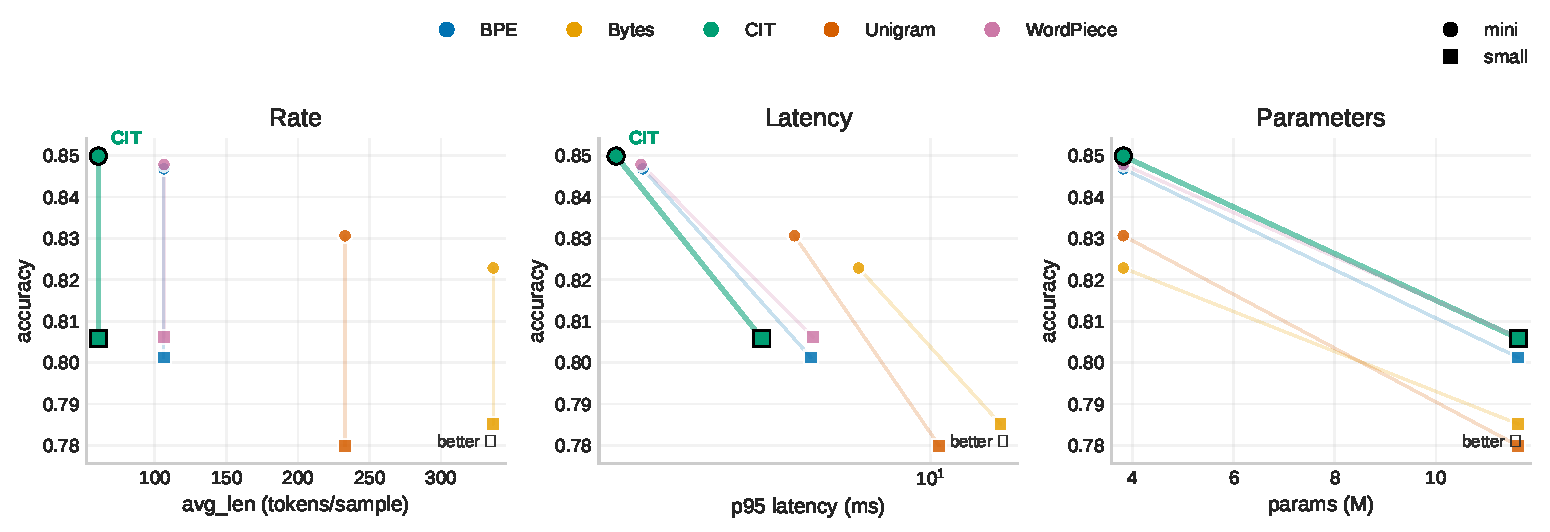
\includegraphics[width=\linewidth]{Figs/e3_pareto_triptych.pdf}
\caption{Accuracy vs.\ efficiency trade-offs on Adult.}
\Description{Three-panel figure comparing tokenizers on the Adult dataset, showing accuracy versus efficiency metrics such as sequence length and latency. CIT achieves similar accuracy with shorter sequences and lower latency.}
\label{fig:e3_pareto}
\end{figure*}

\subsection{Vocabulary-Budget Frontier and Tokenization Time}
\label{sec:exp_frontier}

To directly connect the formulation in Section~\ref{sec:rate_distortion} to practice, we sweep vocabulary budgets $B \in \{256,512,1024,2048,4096\}$ on the Adult serialization and train CIT/BPE/WordPiece tokenizers on the same corpus.
We report interface-level rate (avg./P95 length), surrogate distortion, and tokenization time under deterministic, prefix-emitting execution (Table~\ref{tab:frontier}).
CIT is consistently fast to tokenize and, for moderate and larger vocabularies ($B\ge 512$), yields shorter sequences; beyond $B\ge 1024$ it also reduces distortion, indicating a better empirical frontier under deployment-aligned execution.
At very small budgets, frequency-driven baselines can yield slightly lower distortion, consistent with CIT's design choice of optimizing compression gain (rate) while using distortion as a post hoc interface metric.

\begin{table}[h]
\centering
\scriptsize
\setlength{\tabcolsep}{3.5pt}
\begin{tabular*}{\columnwidth}{@{\extracolsep{\fill}}rlccccc@{}}
\toprule
Vocab & Tokenizer & avg\_len & p95\_len & Distortion $\hat{\Delta}$ & tokenize ms/sample \\
\midrule
256 & CIT & 120.6 & 132 & 0.258 & \textbf{0.03} \\
256 & BPE & \textbf{116.4} & \textbf{128} & \textbf{0.187} & 0.05 \\
256 & WordPiece & 124.5 & 136 & 0.202 & 0.05 \\
\midrule
512 & CIT & \textbf{99.6} & \textbf{111} & 0.206 & \textbf{0.03} \\
512 & BPE & 107.6 & 113 & 0.186 & 0.04 \\
512 & WordPiece & 108.1 & 114 & \textbf{0.178} & 0.05 \\
\midrule
1024 & CIT & \textbf{72.2} & \textbf{82} & \textbf{0.144} & \textbf{0.03} \\
1024 & BPE & 106.8 & 112 & 0.203 & 0.04 \\
1024 & WordPiece & 107.0 & 112 & 0.199 & 0.04 \\
\midrule
2048 & CIT & \textbf{60.5} & \textbf{69} & \textbf{0.138} & \textbf{0.03} \\
2048 & BPE & 106.3 & 111 & 0.206 & 0.09 \\
2048 & WordPiece & 106.4 & 112 & 0.186 & 0.04 \\
\midrule
4096 & CIT & \textbf{58.0} & \textbf{60} & \textbf{0.123} & \textbf{0.03} \\
4096 & BPE & 106.1 & 111 & 0.207 & 0.04 \\
4096 & WordPiece & 106.1 & 111 & 0.189 & 0.04 \\
\bottomrule
\end{tabular*}
\caption{Appendix: vocab-budget frontier sweep. Vocabulary sizes are shown in increasing order. All configurations achieve the same accuracy (0.761); thus only efficiency and distortion metrics are reported. Within each vocabulary budget, tokenizers are ordered with CIT first. Best values (lower is better) are shown in bold.}
\label{tab:appendix_frontier}
\end{table}


\subsection{Generalization to Additional Structured Datasets}
\label{sec:exp_generalization}

Finally, we evaluate on additional public tabular datasets (Adult and Credit-G) under the same drop-in and token-fair protocol.

Across datasets, CIT consistently reduces token rate and surrogate distortion.
Accuracy is maintained on Adult and slightly lower on Credit-G, indicating that efficiency gains do not guarantee uniform accuracy improvements but remain broadly applicable across structured domains.
This pattern is consistent with the interface perspective: CIT is most beneficial when long-tail sequence length and boundary/role brittleness are first-order failure modes, while domains with less high-cardinality string structure may see smaller (or mixed) accuracy changes.
These results reinforce that contract design is a modeling decision and should be tuned to the domain's semantics and to which value spans are truly nuisance versus predictive.

\begin{table}[t]
\centering
\small
\setlength{\tabcolsep}{4pt}
\begin{tabular*}{\columnwidth}{@{\extracolsep{\fill}}lcccc@{}}
\toprule
Tokenizer & Acc. & Avg Len & P95 & Distortion $\hat{\Delta}$ \\
\midrule
\multicolumn{5}{l}{\textit{adult}}\\
CIT        & \textbf{0.842} & \textbf{60.5} & \textbf{69}  & \textbf{0.138} \\
WordPiece  & 0.837 & 106.4 & 112 & 0.186 \\
BPE        & 0.839 & 106.3 & 111 & 0.206 \\
Unigram    & 0.808 & 233.0 & 245 & 0.288 \\
\midrule
\multicolumn{5}{l}{\textit{credit-g}}\\
CIT        & 0.685 & \textbf{99.1} & \textbf{113} & \textbf{0.080} \\
BPE        & \textbf{0.705} & 141.8 & 151 & 0.097 \\
Unigram    & \textbf{0.705} & 321.4 & 339 & 0.170 \\
WordPiece  & 0.670 & 141.7 & 150 & 0.100 \\
\bottomrule
\end{tabular*}
\caption{Additional public tabular benchmarks under token-fair training. Across datasets, CIT consistently reduces sequence length and surrogate distortion, while maintaining comparable accuracy in most cases. These results indicate that the efficiency gains from CIT generalize beyond a single domain.}
\label{tab:e4_uci}
\end{table}


\section{Discussion}
\label{sec:discussion}

Taken together, our results indicate that interface mismatch can induce prefix semantic collapse under prefix-emitting execution, while contract-constrained tokenization improves rate--distortion and robustness trade-offs under strict drop-in budgets.

\paragraph{What changes when tokenization is an interface.}
Tokenization is not only a compression heuristic: under a strict drop-in regime it is a \emph{hard interface} that determines which prefix distinctions reach the model.
For structured streams, interface errors can be causal and irreversible, so fixing the interface can matter more than scaling the same model under the same constraints.

\paragraph{When CIT helps (and why).}
CIT is most appropriate when (i) semantics is role- and boundary-dependent (e.g., key/value structure), (ii) high-cardinality values are frequent and span integrity matters, and (iii) truncation and length tails are first-order concerns.
In this regime, standard subword merges can blur roles for compression, while bytes preserve structure at high rate; CIT prevents collapse with explicit constraints and then recovers efficiency with deployment-aligned gain.

\paragraph{Limitations and failure modes.}
CIT requires an explicit contract; if the contract is underspecified (missing boundaries) or overspecified (forbidding useful merges), performance can degrade.
Typed-value integrity is also a modeling choice: if predictive signal genuinely lies \emph{inside} value strings (e.g., identifier prefixes or checksums that correlate with labels), treating them as atomic can hide useful structure.
Finally, directed semantic distortion is an evaluation tool; practical surrogates depend on the chosen teacher/student capacity and the data distribution.

\paragraph{Towards automatic contracts.}
Many structured deployments already expose schemas, grammars, and validators; reusing them to propose and validate contracts via rate--distortion measurements is a promising direction.

\paragraph{Practical guidance.}
In deployments, the highest-leverage step is to version the serialization and contract alongside the model and audit it under realistic drift operators before vocabulary induction.
When contract design is unclear, start with obvious boundaries and typed spans, measure rate--distortion operating points, and iterate only where the interface collapses semantics.


\section{Conclusion}
\label{sec:conclusion}

We formulated tokenization as controlled interface compression under a drop-in regime and introduced directed semantic distortion as a principled interface metric.
We proposed Controlled Interface Tokenization, aligning feasible constraints, vocabulary induction, and deterministic execution.
Across synthetic and public structured benchmarks, CIT improves rate--distortion trade-offs, downstream accuracy under matched training budgets, and robustness to re-serialization and prefix-limited prediction.
More broadly, the interface perspective suggests that careful, versioned control of serialization and tokenization can be as important as model scaling in structured deployments.
